\documentclass[
    letterpaper,
    man,
    floatsintext,
    british
]{apa6}

\usepackage{longtable}
\usepackage{amssymb}
\usepackage[british]{babel}
\usepackage[utf8]{inputenc}
\usepackage{epstopdf}
\usepackage{csquotes}
\usepackage{placeins}
\usepackage{pgfplots}
\usepackage{pgfplotstable}
\usepackage[hidelinks]{hyperref}
\usepackage{gensymb}
\usepackage[
    style=apa,
    backend=biber,
    sortcites=true,
    sorting=nyt,
%    isbn=false,
    % url=false,
%    doi=false,
%    eprint=false,
    hyperref=false,
    backref=false,
%    firstinits=false,
]{biblatex}
\addbibresource{bibliography.bib}
\usepackage{mathtools}
\pgfplotsset{compat=1.16}

\DeclarePairedDelimiter\abs{\lvert}{\rvert}%
\DeclarePairedDelimiter\norm{\lVert}{\rVert}%

% Swap the definition of \abs* and \norm*, so that \abs
% and \norm resizes the size of the brackets, and the 
% starred version does not.
\makeatletter
\let\oldabs\abs
\def\abs{\@ifstar{\oldabs}{\oldabs*}}
%
\let\oldnorm\norm
\def\norm{\@ifstar{\oldnorm}{\oldnorm*}}
\makeatother

\newcommand*{\Value}{\frac{1}{2}x^2}%

\DeclareLanguageMapping{british}{british-apa}

% maps apacite commands to biblatex commands
\let \citeNP \cite
\let \citeA \textcite
\let \cite \parencite

%%%
% Apa Bib - enable reprint according to apa
%%%

% http://tex.stackexchange.com/questions/139805/how-to-differentiate-between-translated-and-reprinted-work-with-apa-style

\renewbibmacro*{related:reprintfrom}[1]{%
  \entrydata*{#1}{%
    \printtext{\mkbibemph{\printfield[apacase]{title}}}%
    \setunit{\bibpagespunct}%
    \printfield{pages}%
    \setunit{\addcomma\addspace}%
    \bibstring{byauthor}\addspace
    \printnames[apanames][-\value{listtotal}]{editor}%
    \ifnameundef{editor}
      {}
      {\addcomma\addspace
       \usebibmacro{apaeditorstrg}{editor}}
    \printnames[apanames][-\value{listtotal}]{author}%
    \setunit{\addcomma\addspace}%
    \usebibmacro{date}%
    \setunit{\addcomma\addspace}%
    \usebibmacro{location+publisher}%
    \newunit\newblock
    \usebibmacro{related}}}


\DefineBibliographyStrings{british}{
  reprintfrom = {Reprinted from}
}


\bibliography{bibliography}


%%%%%%%%%%%%%%%%%%%%%%%%%%%%%%%%%%%%%%%%%%%%%%%%%%%

\title{Exploring Air Friction and its Effects on Acceleration}
\shorttitle{Exploring Air Friction and its Effects on Acceleration}
\author{David Li, Bert Sun}
\affiliation{John Fraser Secondary School}

\begin{document}

\maketitle

\section{Abstract}
In this experiment we studied the effects of increasing the cross-sectional area of a cart on its acceleration and velocity.
Through this, we proved that air resistance exists and is directly correlated to the cross-sectional area of an object, as well as its shape. Furthermore, we found that air resistance can be decreased by keeping cross-sectional area constant and changing the shape of an object.

\section{Introduction}

Throughout high school physics, we have been calculating the range of projectiles, the velocity of karts, and even the speed of planes - all by assuming that air resistance is negligible.
In this experiment, we set out to prove that air resistance does exist, and that it has a significant impact on acceleration and velocity of an object relative to its cross-sectional area

\section{Background}
\begin{figure}[!h]
  \captionsetup{justification=centering}
  \centering
   

\tikzset{every picture/.style={line width=0.75pt}} %set default line width to 0.75pt        

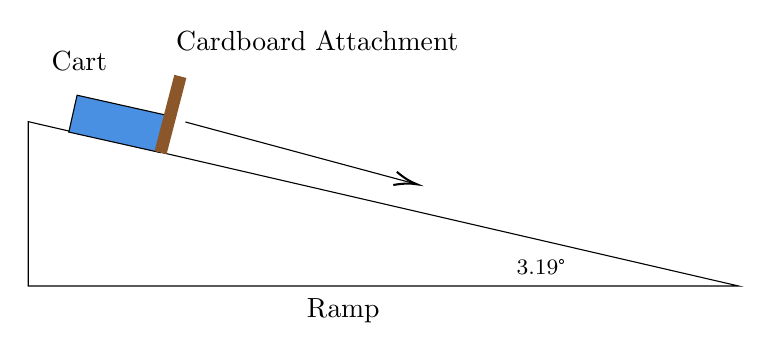
\begin{tikzpicture}[x=0.75pt,y=0.75pt,yscale=-1,xscale=1]
%uncomment if require: \path (0,300); %set diagram left start at 0, and has height of 300

%Shape: Right Triangle [id:dp18569224305294485] 
\draw   (3,189) -- (345.3,268.2) -- (3,268.2) -- cycle ;
%Shape: Rectangle [id:dp7438562411637597] 
\draw  [fill={rgb, 255:red, 74; green, 144; blue, 226 }  ,fill opacity=1 ] (26.54,176.27) -- (70.74,186.17) -- (66.76,203.93) -- (22.56,194.03) -- cycle ;
%Straight Lines [id:da735201395514776] 
\draw [color={rgb, 255:red, 139; green, 87; blue, 42 }  ,draw opacity=1 ][line width=4.5]    (76.3,167.2) -- (66.76,203.93) ;
%Straight Lines [id:da10025482914979356] 
\draw    (78.74,189.17) -- (188.37,218.68) ;
\draw [shift={(190.3,219.2)}, rotate = 195.06] [color={rgb, 255:red, 0; green, 0; blue, 0 }  ][line width=0.75]    (10.93,-3.29) .. controls (6.95,-1.4) and (3.31,-0.3) .. (0,0) .. controls (3.31,0.3) and (6.95,1.4) .. (10.93,3.29)   ;

% Text Node
\draw (237,254) node [anchor=north west][inner sep=0.75pt]   [align=left] {{\fontfamily{}\selectfont {\footnotesize 3.19°}}};
% Text Node
\draw (13,154) node [anchor=north west][inner sep=0.75pt]   [align=left] {{\fontfamily{}\selectfont Cart}};
% Text Node
\draw (73,144) node [anchor=north west][inner sep=0.75pt]   [align=left] {{\fontfamily{}\selectfont Cardboard Attachment}};
% Text Node
\draw (136,273) node [anchor=north west][inner sep=0.75pt]  [align=left] {{\fontfamily{}\selectfont Ramp}};


\end{tikzpicture}
\caption{General experimental setup with a Smart Cart rolling down a ramp. Cross-sectional area of the cart is changed using a cardboard attachment.}
\label{fig:basicramp}
\end{figure}

Figure \ref{fig:basicramp} shows the basic experimental configuration of this experiment. The cart was rolled down
a ramp with an attachment on its front. Said attachment modified the cart's cross-sectional area as well as its
aerodynamic properties. 

We can break down the forces experienced by the cart into components \ref{fig:basicramp} as shown in the free body diagram below.

\begin{figure}[!h]
  \captionsetup{justification=centering}
  \centering
\tikzset{every picture/.style={line width=0.75pt}} %set default line width to 0.75pt        

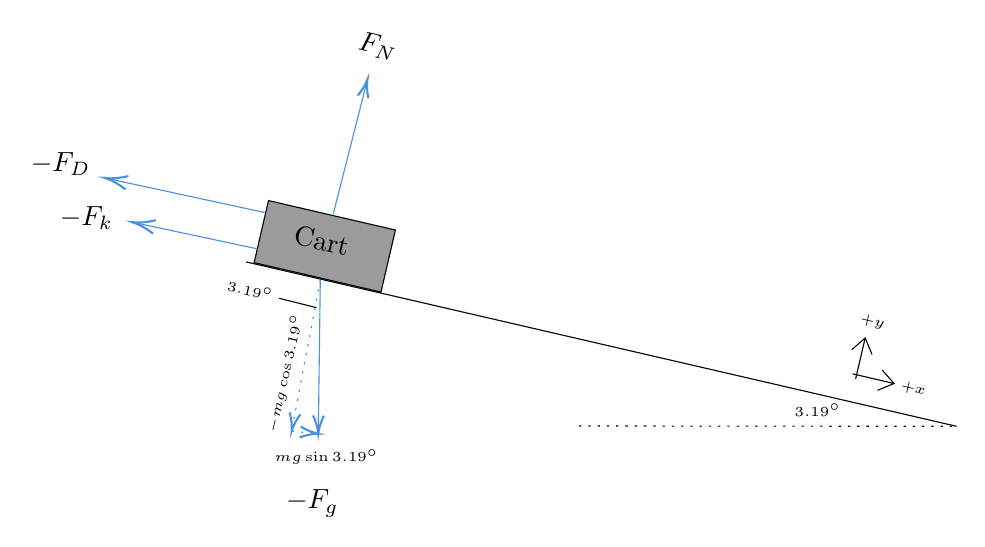
\begin{tikzpicture}[x=0.75pt,y=0.75pt,yscale=-1,xscale=1]
%uncomment if require: \path (0,300); %set diagram left start at 0, and has height of 300

%Straight Lines [id:da25597455715040285] 
\draw    (159,125.8) -- (501.3,205) ;
%Shape: Rectangle [id:dp8095676769699147] 
\draw  [fill={rgb, 255:red, 155; green, 155; blue, 155 }  ,fill opacity=1 ] (169.77,96.25) -- (230.9,110.44) -- (223.96,140.33) -- (162.83,126.14) -- cycle ;
%Straight Lines [id:da9581258174951208] 
\draw [color={rgb, 255:red, 74; green, 144; blue, 226 }  ,draw opacity=1 ]   (200.96,102.71) -- (216.97,39.77) ;
\draw [shift={(217.46,37.83)}, rotate = 464.27] [color={rgb, 255:red, 74; green, 144; blue, 226 }  ,draw opacity=1 ][line width=0.75]    (8.74,-2.63) .. controls (5.56,-1.12) and (2.65,-0.24) .. (0,0) .. controls (2.65,0.24) and (5.56,1.12) .. (8.74,2.63)   ;
%Straight Lines [id:da5736220263506606] 
\draw [color={rgb, 255:red, 74; green, 144; blue, 226 }  ,draw opacity=1 ]   (194.72,134.63) -- (193.78,206.58) ;
\draw [shift={(193.75,208.58)}, rotate = 270.75] [color={rgb, 255:red, 74; green, 144; blue, 226 }  ,draw opacity=1 ][line width=0.75]    (8.74,-2.63) .. controls (5.56,-1.12) and (2.65,-0.24) .. (0,0) .. controls (2.65,0.24) and (5.56,1.12) .. (8.74,2.63)   ;
%Straight Lines [id:da19213091912892] 
\draw [color={rgb, 255:red, 74; green, 144; blue, 226 }  ,draw opacity=1 ] [dash pattern={on 0.84pt off 2.51pt}]  (194.72,134.63) -- (181.27,205.39) ;
\draw [shift={(180.9,207.35)}, rotate = 280.76] [color={rgb, 255:red, 74; green, 144; blue, 226 }  ,draw opacity=1 ][line width=0.75]    (8.74,-2.63) .. controls (5.56,-1.12) and (2.65,-0.24) .. (0,0) .. controls (2.65,0.24) and (5.56,1.12) .. (8.74,2.63)   ;
%Straight Lines [id:da7747687861398798] 
\draw [color={rgb, 255:red, 74; green, 144; blue, 226 }  ,draw opacity=1 ] [dash pattern={on 0.84pt off 2.51pt}]  (180.9,207.35) -- (191.76,208.39) ;
\draw [shift={(193.75,208.58)}, rotate = 185.46] [color={rgb, 255:red, 74; green, 144; blue, 226 }  ,draw opacity=1 ][line width=0.75]    (8.74,-2.63) .. controls (5.56,-1.12) and (2.65,-0.24) .. (0,0) .. controls (2.65,0.24) and (5.56,1.12) .. (8.74,2.63)   ;
%Straight Lines [id:da9726247084266131] 
\draw    (174.9,143.35) -- (192.9,147.85) ;
%Straight Lines [id:da06568273382266154] 
\draw  [dash pattern={on 0.84pt off 2.51pt}]  (319.4,204.85) -- (501.3,205) ;
%Straight Lines [id:da2330937848478929] 
\draw [color={rgb, 255:red, 74; green, 144; blue, 226 }  ,draw opacity=1 ]   (167.9,102) -- (92.85,85.77) ;
\draw [shift={(90.9,85.35)}, rotate = 372.2] [color={rgb, 255:red, 74; green, 144; blue, 226 }  ,draw opacity=1 ][line width=0.75]    (10.93,-3.29) .. controls (6.95,-1.4) and (3.31,-0.3) .. (0,0) .. controls (3.31,0.3) and (6.95,1.4) .. (10.93,3.29)   ;
%Shape: Axis 2D [id:dp4847297973478324] 
\draw  (451.1,179.71) -- (471.16,184.38)(457.24,162.41) -- (452.65,182.15) (465.47,177.92) -- (471.16,184.38) -- (463.21,187.66) (450.79,168.1) -- (457.24,162.41) -- (460.53,170.36)  ;
%Straight Lines [id:da11556239096826859] 
\draw [color={rgb, 255:red, 74; green, 144; blue, 226 }  ,draw opacity=1 ]   (164.4,119.5) -- (106.06,107.07) ;
\draw [shift={(104.1,106.65)}, rotate = 372.03] [color={rgb, 255:red, 74; green, 144; blue, 226 }  ,draw opacity=1 ][line width=0.75]    (10.93,-3.29) .. controls (6.95,-1.4) and (3.31,-0.3) .. (0,0) .. controls (3.31,0.3) and (6.95,1.4) .. (10.93,3.29)   ;

% Text Node
\draw (182.5,106.58) node [anchor=north west][inner sep=0.75pt]  [rotate=-13.1] [align=left] {{\fontfamily{}\selectfont Cart}};
% Text Node
\draw (474.25,181.21) node [anchor=north west][inner sep=0.75pt]  [font=\tiny,rotate=-13.1]  {$+x$};
% Text Node
\draw (454.75,149.21) node [anchor=north west][inner sep=0.75pt]  [font=\tiny,rotate=-13.1]  {$+y$};
% Text Node
\draw (213.64,13.21) node [anchor=north west][inner sep=0.75pt]  [rotate=-12.6]  {$F_{N}$};
% Text Node
\draw (54,71.9) node [anchor=north west][inner sep=0.75pt]    {$-F_{D}$};
% Text Node
\draw (150,132.41) node [anchor=north west][inner sep=0.75pt]  [font=\tiny,rotate=-12.8]  {$3.19\degree $};
% Text Node
\draw (177,234.4) node [anchor=north west][inner sep=0.75pt]    {$-F_{g}$};
% Text Node
\draw (422,192.9) node [anchor=north west][inner sep=0.75pt]  [font=\tiny]  {$3.19\degree $};
% Text Node
\draw (171.5,214.9) node [anchor=north west][inner sep=0.75pt]  [font=\tiny]  {$mg\sin 3.19\degree $};
% Text Node
\draw (166,208) node [anchor=north west][inner sep=0.75pt]  [font=\tiny,rotate=-283]  {$-mg\cos 3.19\degree $};
% Text Node
\draw (68,97.9) node [anchor=north west][inner sep=0.75pt]    {$-F_{k}$};


\end{tikzpicture}
\caption{Free body diagram illustrating various forces acting upon the Smart Cart}
\label{fbdcart}
\end{figure}

In the free body diagram in figure \ref{fbdcart}, the cart is on the ramp, with the forces of air resistance ($F_{D}$) and kinetic friction ($F_{k}$) acting
against the cart in the horizontal direction. The cart is also accelerated down the ramp by the horizontal component of gravity ($mg\sin(3.19\degree)$).


\begin{gather*}
  F_{\textup{net}} = mg\sin(\theta) - F_{K} - kv^2\\
  \\
  ma = mg\sin(\theta) - F_{K} - kv^2\\
\end{gather*}
\begin{equation}
  a = \frac{mg\sin(\theta) - F_{K} - kv^2}{m}
  \label{Eq:acceleration} %the label lets you refer to the equation later
\end{equation}




\section{Methods}
%\section{Methods}
\begin{enumerate}
    \item The wedge was placed underneath the middle of the cardboard so that it made an angle of 43.2 degrees with the horizontal.
    \item The 2 rods were securely taped vertically, 7cm away from the middle of the cardboard. 
    \item The 30cm ruler was taped off to the side of the middle of the cardboard to measure the pullback distance.
    \item The elastic was placed around the 2 rods so that the middle of the elastic lined up with the middle of the cardboard.
    \item A meter stick was placed on the ground where the projectile will land to measure its range. 
        \begin{itemize}
            \item If the range was longer than a meter, the beginning of the meter stick was placed at a fixed offset from the catapult.
        \end{itemize}
    \item Both sides of the elastic were pulled back to the required distance and the projectile was placed in the middle of the elastic.
    \item The projectile was released and its movement was recorded with a camera. The video was analyzed to determine the final range.
    \item Steps 6-7 were repeated 6 more times to minimize experimental error.
    \item Steps 5-8 were repeated with the other pullback distances until there was enough data for all the distances chosen.
\end{enumerate}



\newpage
\section{Results}
\begin{center}
\begin{figure}
    \centering
    \caption{Pullback Distance vs. Projectile Range}
    \label{fig:graph1}
    \pgfplotstableread[col sep = comma]{data.csv}\loadedtable
    \begin{tikzpicture}
    \begin{axis}[
        xlabel=Pullback Distance (cm), % label x axis
        ylabel=Distance Travelled (cm), % label y axis
        axis lines=left, %set the position of the axes
        clip=false,
        width=12cm
    ]

            \addplot[scatter, only marks] table [x=Pull Back Distance (cm), y=Distance, col sep=comma] {\loadedtable};
            \addplot [color=black, domain=1.5:15.5, mark=none smooth, thick] {0.91*x^2+17.9*x-51.3}  node[above,pos=1] {$0.91x^2+17.9x-51.3$};
    \end{axis}
\end{tikzpicture}
\\
\small\textit{$R^2$ = 0.992}
\end{figure}
\end{center}

% \begin{table}[H]
  \caption{\textit{K} values relative to cross-sectional area and the shape of the attachment}
  \centering
  \label{table:results}
  \begin{tabular*}{\textwidth}{l@{\extracolsep{\fill}}llll}
  \thickline
  \textbf{Attachment}   & \textbf{Length (cm)} & \textbf{Width (cm)} & \textbf{Area ($\textup{cm}^2$)} & \textbf{K} \\ \thickline
  None                  & 3.4             & 8.5            & 33.85                                 & 0.002      \\
  Orange                & 29              & 33             & 957                                   & 0.184      \\
  Cardboard             & 12              & 20.75          & 249                                   & 0.105      \\
  Cardboard             & 15.78           & 15.78          & 249                                   & 0.109      \\
  Orange Pocket         & 29              & 33             & 957                                   & 0.198      \\
  Equilateral Wedge     & 9.4             & 26.5           & 249                                   & 0.087      \\
  Sharp Wedge           & 9.4             & 26.5           & 249                                   & 0.050      \\
  Sharp Wedge on Orange & 29              & 33             & 957                                   & 0.127     
  \\ \thickline
  \end{tabular*}
  \end{table}

\section{Discussion}
\subsection{Methodology}
One unique part of our methodology that proved crucial to the statistical
significance and accuracy of our data was the addition of a 250g weight on top of the
Smart Cart. Adding the various cardboard attachments used to modify the aerodynamic properties of the
Smart Cart would increase the total weight of our modified Smart Cart system. It would be possible to
account for the variance in weight by measuring each cardboard attachment along with the tape used to
affix it; however, a lack of time meant that it would be more efficient to make the additional weight
negligible by increasing the overall weight of the Smart Cart itself. Although this may introduce some
variance into our results, the relative effect of the additional weight is acceptable given how little
the attachments weighed relative to the weighted Smart Cart.

\subsection{Air Resistance}
A major goal of this experiment was to determine whether or not air resistance actually existed, or if 
it had enough of an effect to affect our data in a manner that was statistically significant. If air resistance
were to exist and be statistically significant with respect to the data collected, then there should be a statistically significant
decrease in acceleration due to the increasing drag forces. After collecting multiple sets of
data and removing outliers based on inter-quartile ranges, the data for each trial were individually plotted on a graph.
Specifically, when acceleration relative to time was plotted for each trial, as well as a linear regression for acceleration relative to time,
it becomes clear that when cross-sectional area is increased, there is a time-dependent, increasing drag force that decreases acceleration.
Referring to \ref{chart:cardboard12x20.75}, \ref{chart:cardboard15.78x15.78}, \ref{chart:equilateralwedge}, \ref{chart:orange}, \ref{chart:orangepocket}, \ref{chart:sharpwedge}, and \ref{chart:sharpwedgeonorange},
each of their respective linear regressions of acceleration all have negative slopes and decrease with respect to time - signifying an overall deceleration.
Furthermore, when referring to the base case, \ref{chart:nothing}, it can be seen that the slope of the linear regression of acceleration is
practically zero. The base case did not have a cardboard attachment or an increased cross-sectional area.
This shows that increasing cross-sectional area will affect the aerodynamic properties of the cart,
which will create drag forces that decelerate the cart.

\subsection{Calculating the Drag Coefficient (\textit{K})}
To calculate the drag coefficient for a given time, we can use equation \ref{Eq:K}.
Since all the variables needed to solve for \textit{K} at a given time are known, then 
these values can be substituted to solve for \textit{K} at a given time - with the exception of $F_{k}$ from
equation \ref{Eq:F}. 

\subsection{Calculating the Force of Kinetic Friction ($F_{k}$)}
The friction forces on the cart are a system
composed of static friction from the wheels on the ramp, and kinetic friction on the axles. It
becomes difficult to find kinetic friction since it presents two unknowns: $F_{k}$ and \textit{K}.
To determine $F_{k}$ without needing to use two unknown variables, we let $K = 0$ in the base case
where the cart had no additional attachments affecting its cross-sectional area. We were able to set \textit{K}
to zero in this case because in \ref{chart:nothing}, the linear regression of acceleration for the base case was equal to zero, thus showing
that the deceleration due to air resistance was also zero. To find for $F_{k}$ given \textit{K}, we can solve
for $F_{k}$ as a function of time by dividing acceleration by the mass of the cart and then average over the time interval
of the respective trial. This will give us a numeric value for $F_{k}$ if it is needed in other calculations.
For the purposes of this experiment, $F_{k}$ is included in the variable $F$\footnote{$F$ is the average force measured by the Smart Cart for the base case, as the average
force experienced by the cart when air resistance is negligible would only be the component of gravity down the ramp, and $-F_{k}$} from \ref{Eq:F}, and not directly
substituted into any calculations.

\subsection{The Correlation Between Shape, Cross-Sectional Area, Angle of the Wedge, and \textit{K}}

\subsubsection{Cross-Sectional Area}
From the results in \ref{table:results}, we are able to see that for most cases, an increase in \textit{K}
correlates to an increase in the overall cross-sectional area of that attachment. We also see that changing the dimensions
of an attachment, but keeping surface area constant (as shown in both cardboard trials) does not affect \textit{K} in a
significant manner. In fact, the change in \textit{K} for this case is marginal, and one could argue that it is not a statistically significant
change.

\subsubsection{Angle of the Wedge}
% for wedge, statistically insignificant, force of air friction couldn't be measured properly
Another interesting observation were the effects of adding an equilateral wedge onto the Smart Cart system. The equilateral wedge was of the same
cross-sectional area as the cardboard, however, it had a significantly lower drag coefficient. This is due to the shape of the
attachment itself. A wedge is able to "cut" through the air, which creates less turbulence and frictional drag around the surfaces
of the attachment compared to a fully flat piece of cardboard. The shape of the wedge also redirects the air around the attachment
instead of directly impacting the air, causing less deceleration upon the Smart Cart system.
When the angle of the sharp part of the wedge facing forward was changed so that it was sharper, we see that \textit{K}
decreases relative to a normal equilateral wedge. Making the leading edges of the wedge have a smaller angle relative
to the ramp results in less force being used to push the air out of the way. Normally, for an attachment that is flat, the air directly
creates a normal force against that attachment, pushing it up the ramp. With a sharp wedge, the sharper angles redirect that normal force
so that it points outwards from the edge, resulting in less push-back against the cart in the horizontal direction.

Linear regressions of the acceleration of both wedges are of the same order of magnitude as that of the cart with no attachments.
However, these figures do carry a certain statistical insignificance due to the almost harmonic fluctuation of acceleration in these cases.
Therefore, it can be said that adding these wedges make the cart have no air friction, or that air friction cannot be measured properly due to the 
inaccuracy of the cart's measurements.

A sharp wedge was also added onto the flat orange cardboard attachment. Even though the sharp wedge did not fit over the entire
surface of the orange attachment, it still decreased its drag coefficient by 30.97\%. The sharp wedge was attached to the bottom
of the orange attachment, which reduced the force required to redirect air around that edge. Furthermore, for the area in which the
sharp wedge did occupy, it reduced the normal force of air resistance on those areas, thereby reducing the overall deceleration
caused by the force of air resistance. This shows that attaching even a small wedge onto a larger surface can make that surface more
aerodynamic.

\subsubsection{Shape}
Both wedge, and flat cardboard shapes and their relation to \textit{K} have been previously discussed. When we flipped
the orange cardboard attachment (top cover of a shoebox) over so that the raised edges face forward, it was observed that the
\textit{K} value slightly increased relative to the flat side of the orange cardboard attachment. These attachments both have the
same cross-sectional area, however, the overall shape of the "pocketed" orange attachment with its raised edges was more
conducive to creating turbulence and frictional drag against the air. It can be theorized that the raised edges effectively
trap some of the air impacting the attachment, thereby creating a pocket of air that creates more air resistance and decelerating the Smart Cart system.

\subsubsection{General Conclusions}
Through these trials, it can be shown that increasing the cross-sectional area of the Smart Cart increases the drag coefficient \textit{K}
and decelerates the cart. Changing the dimensions while retaining the same cross-sectional area does not appear
to affect air resistance and the \textit{K} value. It can also be shown that changing the angle at which the attachment impacts the air can
decrease air resistance, and making said angle sharper, or smaller relative to the ramp, can further decrease air resistance.
Finally, changing the shape of the attachment by adding raised edges also causes more air resistance, thereby increasing \textit{K} and
causing deceleration.

\nocite{*}
\printbibliography

\newpage
\appendix
\title{Sample Calculations}
\section{Trial Charts}
\begin{center}
  \begin{figure}[H]
      \centering
      \caption{Raw Data Collected from Smart Cart and Calculated \textit{K} value - No Attachment}
      \label{chart:nothing}
      \pgfplotstableread[col sep = comma]{data/nothing.csv}\loadedtable
      \begin{tikzpicture}
      \begin{axis}[
          xlabel=Time (s), % label x axis
          % ylabel=Distance Travelled (cm), % label y axis
          axis lines=left, %set the position of the axes
          clip=false,
          width=16cm,
          height=8.5cm,
      ]
  
              \addplot[color=blue,mark=none] table [x=Time (s), y=K, col sep=comma] {\loadedtable};
              \addplot[color=red,mark=none] table [x=Time (s), y=Force (N), col sep=comma] {\loadedtable};
              \addplot[color=yellow,mark=none] table [x=Time (s), y=Position (m), col sep=comma] {\loadedtable};
              \addplot[color=green,mark=none] table [x=Time (s), y=Velocity (m/s), col sep=comma] {\loadedtable};
              \addplot[color=orange,mark=none] table [x=Time (s), y=Acceleration (m/s2), col sep=comma] {\loadedtable};
              \addplot [color=black, domain=0:1.5, mark=none smooth, thick] {(2.37*10^-03)*x+0.509}  node[above,pos=1] {$2.37E-03*x + 0.509$};
              \legend{K, Force (N), Position (m), Velocity (m/s), Acceleration (m/s$^2$)}
      \end{axis}
  \end{tikzpicture}
  \\
  \end{figure}
  \end{center}
  
\begin{center}
  \begin{figure}[H]
      \centering
      \caption{Raw Data Collected from Smart Cart and Calculated \textit{K} value - Orange}
      \label{chart:orange}
      \pgfplotstableread[col sep = comma]{data/orange.csv}\loadedtable
      \begin{tikzpicture}
      \begin{axis}[
          xlabel=Time (s), % label x axis
          % ylabel=Distance Travelled (cm), % label y axis
          axis lines=left, %set the position of the axes
          clip=false,
          width=16cm,
          height=8.5cm,
      ]
  
              \addplot[color=blue,mark=none] table [x=Time (s), y=K, col sep=comma] {\loadedtable};
              \addplot[color=red,mark=none] table [x=Time (s), y=Force (N), col sep=comma] {\loadedtable};
              \addplot[color=yellow,mark=none] table [x=Time (s), y=Position (m), col sep=comma] {\loadedtable};
              \addplot[color=green,mark=none] table [x=Time (s), y=Velocity (m/s), col sep=comma] {\loadedtable};
              \addplot[color=orange,mark=none] table [x=Time (s), y=Acceleration (m/s2), col sep=comma] {\loadedtable};
              \addplot [color=black, domain=0:1.45, mark=none smooth, thick] {(-0.0592*x)+0.467}  node[above,pos=1] {$-0.0592x + 0.467$};
              \legend{K, Force (N), Position (m), Velocity (m/s), Acceleration (m/s$^2$)}
      \end{axis}
  \end{tikzpicture}
  \\
  \end{figure}
  \end{center}
  
\begin{center}
  \begin{figure}[H]
      \centering
      \caption{Raw Data Collected from Smart Cart and Calculated \textit{K} value - Cardboard (12 x 20.75)}
      \label{chart:cardboard12x20.75}
      \pgfplotstableread[col sep = comma]{data/cardboard12x20.75.csv}\loadedtable
      \begin{tikzpicture}
      \begin{axis}[
          xlabel=Time (s), % label x axis
          % ylabel=Distance Travelled (cm), % label y axis
          axis lines=left, %set the position of the axes
          clip=false,
          width=16cm,
          height=8.5cm,
          legend pos=south east
      ]
  
              \addplot[color=blue,mark=none] table [x=Time (s), y=K, col sep=comma] {\loadedtable};
              \addplot[color=red,mark=none] table [x=Time (s), y=Force (N), col sep=comma] {\loadedtable};
              \addplot[color=yellow,mark=none] table [x=Time (s), y=Position (m), col sep=comma] {\loadedtable};
              \addplot[color=green,mark=none] table [x=Time (s), y=Velocity (m/s), col sep=comma] {\loadedtable};
              \addplot[color=orange,mark=none] table [x=Time (s), y=Acceleration (m/s2), col sep=comma] {\loadedtable};
              \addplot [color=black, domain=0:1.54, mark=none smooth, thick] {(-0.073)*x+0.496};
              \legend{K, Force (N), Position (m), Velocity (m/s), Acceleration (m/s$^2$), $-0.073x + 0.496$}
      \end{axis}
  \end{tikzpicture}
  \\
  \end{figure}
  \end{center}
  
\begin{center}
  \begin{figure}[H]
      \centering
      \caption{Raw Data Collected from Smart Cart and Calculated \textit{K} value - Cardboard (15.78 x 15.78)}
      \label{chart:cardboard15.78x15.78}
      \pgfplotstableread[col sep = comma]{data/cardboard15.78x15.78.csv}\loadedtable
      \begin{tikzpicture}
      \begin{axis}[
          xlabel=Time (s), % label x axis
          % ylabel=Distance Travelled (cm), % label y axis
          axis lines=left, %set the position of the axes
          clip=false,
          width=16cm,
          height=8.5cm,
          legend pos=south east
      ]
  
              \addplot[color=blue,mark=none] table [x=Time (s), y=K, col sep=comma] {\loadedtable};
              \addplot[color=red,mark=none] table [x=Time (s), y=Force (N), col sep=comma] {\loadedtable};
              \addplot[color=yellow,mark=none] table [x=Time (s), y=Position (m), col sep=comma] {\loadedtable};
              \addplot[color=green,mark=none] table [x=Time (s), y=Velocity (m/s), col sep=comma] {\loadedtable};
              \addplot[color=orange,mark=none] table [x=Time (s), y=Acceleration (m/s2), col sep=comma] {\loadedtable};
              \addplot [color=black, domain=0:1.63, mark=none smooth, thick] {(-0.023)*x+0.478};
              \legend{K, Force (N), Position (m), Velocity (m/s), Acceleration (m/s$^2$), $-0.023x + 0.478$}
      \end{axis}
  \end{tikzpicture}
  \\
  \end{figure}
  \end{center}
  
\begin{center}
  \begin{figure}[H]
      \centering
      \caption{Raw Data Collected from Smart Cart and Calculated \textit{K} value - Equilateral Wedge}
      \label{chart:equilateralwedge}
      \pgfplotstableread[col sep = comma]{data/equilateralwedge.csv}\loadedtable
      \begin{tikzpicture}
      \begin{axis}[
          xlabel=Time (s), % label x axis
          % ylabel=Distance Travelled (cm), % label y axis
          axis lines=left, %set the position of the axes
          clip=false,
          width=16cm,
          height=8.5cm,
          legend pos=south east
      ]
  
              \addplot[color=blue,mark=none] table [x=Time (s), y=K, col sep=comma] {\loadedtable};
              \addplot[color=red,mark=none] table [x=Time (s), y=Force (N), col sep=comma] {\loadedtable};
              \addplot[color=yellow,mark=none] table [x=Time (s), y=Position (m), col sep=comma] {\loadedtable};
              \addplot[color=green,mark=none] table [x=Time (s), y=Velocity (m/s), col sep=comma] {\loadedtable};
              \addplot[color=orange,mark=none] table [x=Time (s), y=Acceleration (m/s2), col sep=comma] {\loadedtable};
              \addplot [color=black, domain=0:0.88, mark=none smooth, thick] {(-6.78*10^-3)*x+0.489};
              \legend{K, Force (N), Position (m), Velocity (m/s), Acceleration (m/s$^2$), $-6.78E-3*x + 0.489$}
      \end{axis}
  \end{tikzpicture}
  \\
  \end{figure}
  \end{center}
  
\begin{center}
  \begin{figure}[H]
      \centering
      \caption{Raw Data Collected from Smart Cart and Calculated \textit{K} value - Orange with Pocket}
      \label{chart:orangepocket}
      \pgfplotstableread[col sep = comma]{data/orangepocket.csv}\loadedtable
      \begin{tikzpicture}
      \begin{axis}[
          xlabel=Time (s), % label x axis
          % ylabel=Distance Travelled (cm), % label y axis
          axis lines=left, %set the position of the axes
          clip=false,
          width=16cm,
          height=8.5cm,
      ]
  
              \addplot[color=blue,mark=none] table [x=Time (s), y=K, col sep=comma] {\loadedtable};
              \addplot[color=red,mark=none] table [x=Time (s), y=Force (N), col sep=comma] {\loadedtable};
              \addplot[color=yellow,mark=none] table [x=Time (s), y=Position (m), col sep=comma] {\loadedtable};
              \addplot[color=green,mark=none] table [x=Time (s), y=Velocity (m/s), col sep=comma] {\loadedtable};
              \addplot[color=orange,mark=none] table [x=Time (s), y=Acceleration (m/s2), col sep=comma] {\loadedtable};
              \addplot [color=black, domain=0:1.49, mark=none smooth, thick] {(-0.0846)*x+0.488}  node[above,pos=1] {$-0.0846x + 0.488$};
              \legend{K, Force (N), Position (m), Velocity (m/s), Acceleration (m/s$^2$)}
      \end{axis}
  \end{tikzpicture}
  \\
  \end{figure}
  \end{center}
  
\begin{center}
  \begin{figure}[H]
      \centering
      \caption{Raw Data Collected from Smart Cart and Calculated \textit{K} value - Sharp Wedge}
      \label{chart:sharpwedge}
      \pgfplotstableread[col sep = comma]{data/sharpwedge.csv}\loadedtable
      \begin{tikzpicture}
      \begin{axis}[
          xlabel=Time (s), % label x axis
          % ylabel=Distance Travelled (cm), % label y axis
          axis lines=left, %set the position of the axes
          clip=false,
          width=16cm,
          height=8.5cm,
      ]
  
              \addplot[color=blue,mark=none] table [x=Time (s), y=K, col sep=comma] {\loadedtable};
              \addplot[color=red,mark=none] table [x=Time (s), y=Force (N), col sep=comma] {\loadedtable};
              \addplot[color=yellow,mark=none] table [x=Time (s), y=Position (m), col sep=comma] {\loadedtable};
              \addplot[color=green,mark=none] table [x=Time (s), y=Velocity (m/s), col sep=comma] {\loadedtable};
              \addplot[color=orange,mark=none] table [x=Time (s), y=Acceleration (m/s2), col sep=comma] {\loadedtable};
              \addplot [color=black, domain=0:0.88, mark=none smooth, thick] {(-9.67*10^-4)*x+0.457}  node[above,pos=1] {$-9.67E-4*x + 0.457$};
              \legend{K, Force (N), Position (m), Velocity (m/s), Acceleration (m/s$^2$)}
      \end{axis}
  \end{tikzpicture}
  \\
  \end{figure}
  \end{center}
  
\begin{center}
  \begin{figure}[H]
      \centering
      \caption{Raw Data Collected from Smart Cart and Calculated \textit{K} value - Sharp Wedge on Orange}
      \label{chart:sharpwedgeonorange}
      \pgfplotstableread[col sep = comma]{data/sharpwedgeonorange.csv}\loadedtable
      \begin{tikzpicture}
      \begin{axis}[
          xlabel=Time (s), % label x axis
          % ylabel=Distance Travelled (cm), % label y axis
          axis lines=left, %set the position of the axes
          clip=false,
          width=16cm,
          height=8.5cm,
          legend pos=south east
      ]
  
              \addplot[color=blue,mark=none] table [x=Time (s), y=K, col sep=comma] {\loadedtable};
              \addplot[color=red,mark=none] table [x=Time (s), y=Force (N), col sep=comma] {\loadedtable};
              \addplot[color=yellow,mark=none] table [x=Time (s), y=Position (m), col sep=comma] {\loadedtable};
              \addplot[color=green,mark=none] table [x=Time (s), y=Velocity (m/s), col sep=comma] {\loadedtable};
              \addplot[color=orange,mark=none] table [x=Time (s), y=Acceleration (m/s2), col sep=comma] {\loadedtable};
              \addplot [color=black, domain=0:1.54, mark=none smooth, thick] {(-0.0384)*x+0.476};
              \legend{K, Force (N), Position (m), Velocity (m/s), Acceleration (m/s$^2$), $-0.0384x + 0.476$}
      \end{axis}
  \end{tikzpicture}
  \\
  \end{figure}
  \end{center}
  

\title{Sample Calculations}
\section{Sample Calculations}
\subsection{K Value}
\label{sampleCalc}
\begin{gather*}
    F = 0.2527074\textup{N} \\
    a(t) = 0.505 \: \frac{\textup{m}}{\textup{s}^2} \\
    v(t) = 0.23 \: \frac{\textup{m}}{\textup{s}} \\
    m = 0.495 \textup{kg}
\end{gather*}
\begin{gather*}
    K = \frac{F - a(t)m}{v(t)^2} \\\\
    K = \frac{0.2527074\textup{N} - 0.505 \: \frac{\textup{m}}{\textup{s}^2} *  0.495 \textup{kg}}{(0.23 \: \frac{\textup{m}}{\textup{s}})^2} \\\\
    K = 0.05165217381
\end{gather*}



\end{document}
